Apromore is a Web-based advanced process analytics platform, developed by the BPM community under an open-source initiative.\footnote{\url{http://apromore.org}} Apromore was originally conceived as an advanced process model repository. However, today it offers a wide range of features which go beyond those for managing large process model collections, and include a variety of state-of-the-art process mining techniques. These are techniques for the automated discovery of BPMN models, for the conformance checking of BPMN models against event logs, the replaying of event logs on top of BPMN models, the detection and characterization of process drifts from event logs, the visual analysis of process performance, and many others. 

All these features are exposed through a Web portal, and organized according to the phases of the BPM lifecycle: discovery, analysis, redesign, implementation and monitoring. These features can also be accessed as external Web services by third-party BPM software environments, such as ProM (for process mining) and WoPeD (for process modeling and verification).

From a technology viewpoint, Apromore relies on four core technologies: Spring, ZK, OSGi and Eclipse Virgo. Spring provides a simplified management of Java-based enterprise applications through the use of Java annotations and XML configurations. ZK is an AJAX framework used for Apromore's main Web interface (the \emph{Portal}). OSGi provides a flexible framework for managing component dependencies through plugin bundles. Finally, Eclipse Virgo is a Web server based on the OSGi component model.

To equip Apromore with predictive process monitoring capabilities, we have wrapped the two core components of Nirdizati into two OSGi plugin bundles for Apromore: Training and Runtime. Each bundle is a set of OSGi plugins which encapsulate the logic or the user interface (UI) of the various functions offered by Nirdizati. For example, the runtime predictor is a logic plugin, while the runtime dashboard is a portal plugin (UI). These two bundles are accessible from the Monitoring menu of the Apromore Portal (see Figure~\ref{fig:apromore-menus}). One can select an event log stored in the repository, and use it to train, tune and test a variety of predictive models, by launching the training plugin bundle. Next, the runtime bundle can be used to stream an event log from the repository, or hook into a live external stream, in order to generate predictions as process cases unfold.    

\begin{figure}[t!]%[H]
	\centering
	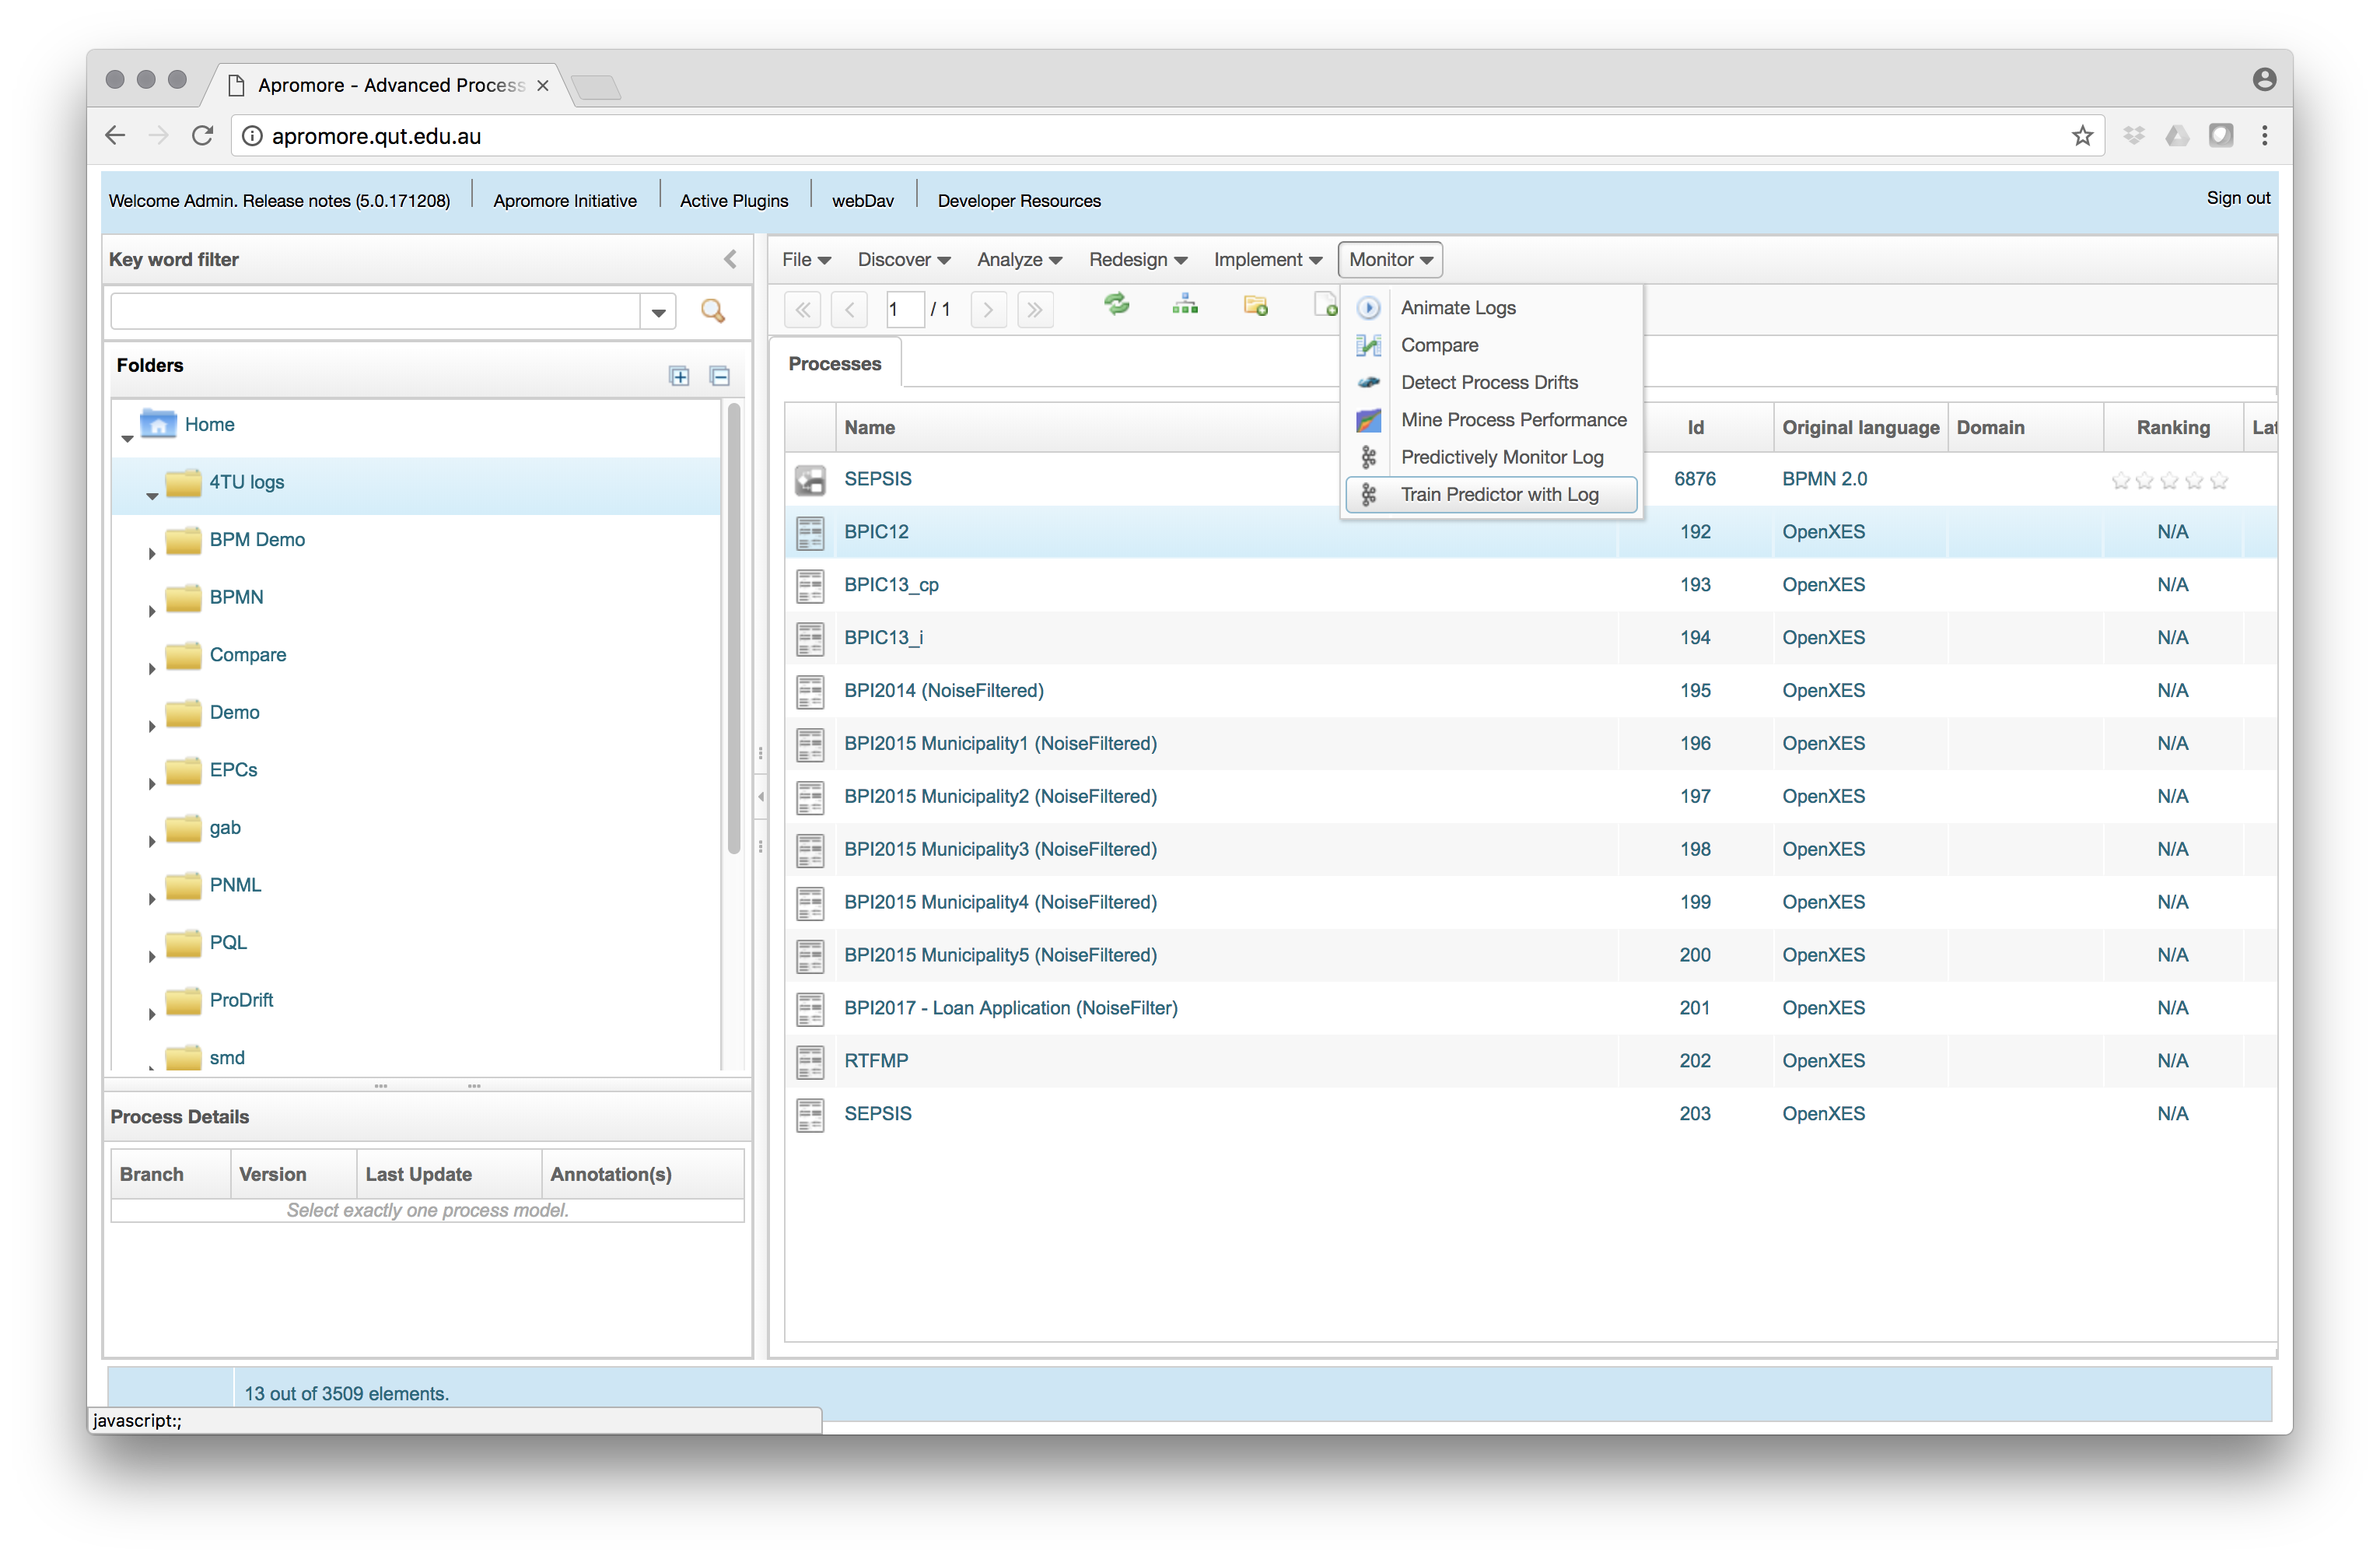
\includegraphics[width=\textwidth]{img/apromore-menus}
	%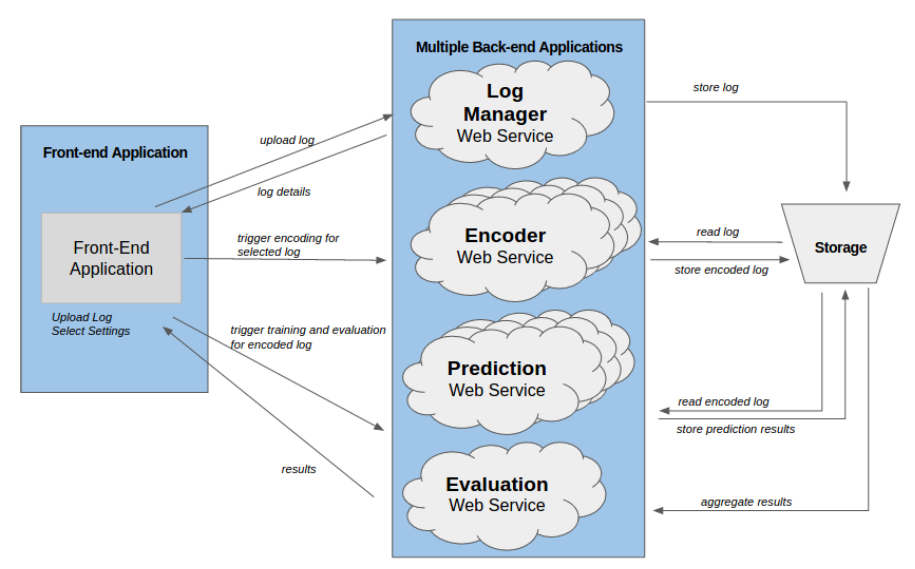
\includegraphics[width=0.7\textwidth]{img/nirdizati-training}
	\vspace{-2\baselineskip}
	\caption{Apromore's Portal with predictive monitoring functionality highlighted.}
	\label{fig:apromore-menus}
\end{figure}

In the next sections, we introduce a working example and use this to describe the functionality of the training and runtime plugins in detail.

